% status: 75
% chapter: Amazon

\title{AWS CloudTrail}

\author{Michael Robinson}
\affiliation{%
  \institution{Indiana University}
  \country{USA}}
\email{micbrobi@umail.iu.edu}


% The default list of authors is too long for headers}
\renewcommand{\shortauthors}{M. Robinson}


\begin{abstract}
The AWS CloudTrail service~\cite{hid-sp18-518-CloudTrail} is an activity 
recording service provided by Amazon Web Services. The service allows you to 
track the history of account usage for your AWS instances. The service is not 
on by default yet when configured, it will record all API calls from all 
sources like the console, CLE, SDKs or CloudFormation. The data is written 
into an S3 bucket via JSON and would include attributes like user, IP address, 
timestamp and the action the user took.
\end{abstract}

\keywords{hid-sp18-518, CloudTrail}

\maketitle

\section{Introduction}

Your API is finally working. After weeks of learning Docker, AWS Lambda and 
other Cloud technologies, you feel the pride of seeing your code finally 
providing a service. And that service is on the Internet! Yet, a few days 
later, you are notified by AWS that your AWS bill is about to reach the cap 
you set for it. That obviously can’t be right. As you log into your AWS 
account to check on what is going on, you notice containers running that you 
don’t recognize. How is this possible? Who did this? That is where 
CloudTrail~\cite{hid-sp18-518-CloudTrail} can help.

As cloud technologies are quickly adopted, one of the common mistakes is 
skipping past features related to security. To cover the aspect of
logging and monitoring, both features that are critical to ensuring 
appropriate use, and the intent is to help build understanding of how these 
features can help you keep your system uptime high, your bills low and provide 
you certainty that you know when changes occur.

CloudTrail is a scalable, extensible and simplied logging service available 
in AWS to be used to log all actions taken by multiple aspects of interacting
with AWS. In AWS, one of the primary means of providing logging is through AWS 
CloudTrail. Amazon explains it as a service that enables governance, 
compliance, operational auditing, and risk auditing of your AWS 
account~\cite{hid-sp18-518-CloudTrail-user-guide}. To simplify, AWS provides 
a logging service that can be used to meet logging requirements, either ones
you design personally or requirements that are directed by a higher entity 
such as government or a regulatory body such as PCI-DSS, HIPAA or NIST
Security Technical Implementation Guides.

\section{How it works}

CloudTrail will record activity, based on your configuration, into an 
AWS S3 bucket~\cite{hid-sp18-518-CloudTrail-log-example}.
The JSON-formatted log files are compressed before they are written into an 
S3 bucket. The convention for storing the files consists of two 
parts, path and filename. The path will follow a convention of 
account/region/date and each day will have its own path.  The filename of the 
compressed file follows a convention of account/region/timestamp. 

\begin{figure}[!ht]
	\centering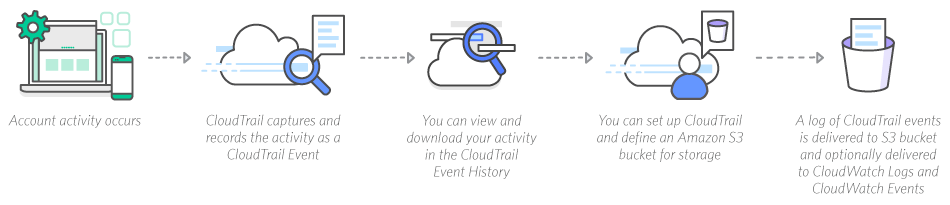
\includegraphics[width=\columnwidth]{../images/Cloudtrail-How-it-works.png}
	\caption{KNIME Architecture~\cite{hid-sp18-518-CloudTrail-CloudFormation-Image}}
 	\label{fig:CloudTrail}
\end{figure}

The default path of account to region may not work well for a multi-account, 
multi-region AWS instance. There are options to define logging for multi-region 
where the configuration can be applied to all known existing regions and even 
configured to include new ones when they come online by 
default~\cite{hid-sp18-518-CloudTrail-global-events}. Additionally, 
for multi-user situations, you can leverage AWS Identity and Access 
Management~\cite{hid-sp18-518-CloudTrail-IAM} to set global logging for all 
accounts as well.

To manage CloudTrail, you can use the AWS command line interface, RESTful APIs
or a software development kit for Python, Java or multiple other languages. 
These methods will allow you to make view the existing logs, which are natively 
built in for you for the first 90 days. The management interfaces also allow
you configure which S3 bucket to use, prefixes you may wish for organization, 
encryption keys to be used as well as more complex features like custom event
notifications to solutions like email, Slack channels or a text message.

The AWS command line environment is the most full-featured. To do so, you first 
will need credentials for an active AWS account. As credential management can 
be its own comlex topic,  the AWS configuration guide should be leveraged to 
provide a step by step to configure credentials. The simplest way to set up a 
trail is to use a command as follows: 

aws cloudtrail create-trail --name my-trail --s3-bucket-name my-bucket

The two parameters to declare are name, which is the unique name you want to 
provide to the trail and the second is the s3 bucket to use.

If you choose to use the RESTful API support, these are a few of
the actions currently available to be called.

\begin{itemize}
\item AddTags
\item CreateTrail
\item DeleteTrail
\item LookupEvents
\item StartLogging
\item StopLogging
\end{itemize}

If you used the API call, the response from a successful query will respond with 
a 200 HTTP status code and a JSON blob with the requested content. For example,
when using LookupEvents, the response back for a query related to a user would be 
include the following details.

\begin{itemize}
\item eventVersion
\item userIdentity
\item type
\item principalId
\item arn
\item userName
\item eventTime
\item eventSource
\item sourceIPAddress
\item userAgent
\item requestParameters
\end{itemize}

Another solution you can use are called AWS Quick 
Starts~\cite{hid-sp18-518-CloudTrail-Quick-Starts} which can reduce error 
caused by manual implementation. The command create-subscription will automate the 
creation of an S3 bucket and will begin the login. AWS provides these prebuilt
solutions for customers who may not feel comfortable with using AWS or want
to try a solution out before configuring on their own.

Advanced CloudTrail configurations can be managed using 
CloudFormation~\cite{hid-sp18-518-CloudTrail-CloudFormation} which allows you
to define multiple aspects of an AWS instance in a text file using YAML or 
JSON formatted files. A visual editor is available in AWS to build a template
or community-provided templates are also available. For CloudTrail, the use
of CloudFormation ensures that all instances stood up that are using a template
will have CloudTrail defined and set up as well.

To ensure no one can  accidentally delete your CloudTrail logs,
it is important to leverage features in Identity and Access Management. With 
Identity and Access Management, you can grant access per user on who is 
authorized to read logs stored in the CloudTrail S3 bucket 
or who can make changes to the CloudTrail configuration. It is also recommended 
to leverage features like Multi-Factor Authentication, which can be used to 
ensure that a request to delete an S3 bucket for CloudTrail logs is 
legitimate~\cite{hid-sp18-518-CloudTrail-user-guide}. 

Another aspect where Identity and Access Management can help you with CloudTrail 
is ensuring the logs are owned by a service account. Access requests to the log 
data can be controlled by only authorizing access by log analysis and correlation 
service accounts and a human would never had direct access to the logs stored in 
S3. This helps ensure access control is not lost if your organizational use of 
AWS Identity and Access Management continues to grow. 

To ensure no one can intentionally or accidentally delete your CloudTrail logs,
 it is important to leverage Identity and Access Management to limit access 
per user on who is authorized to read logs stored in the CloudTrail S3 bucket 
or who can make changes to the CloudTrail configuration. 

The CloudTrail log integrity solution is a process which will create hashes 
for the current log metadata and appends some information from the previous log 
archive. That way you can walk back the integrity of your logs and quickly 
identify which log was tampered with. The log validation service also provides 
you a tool to assist with validation and you just need to provide it a time 
range to validate~\cite{hid-sp18-518-CloudTrail-log-sharing}.

\section{How to view the logs}

The most common method to review the logs is with the AWS command line interface. 
While useful, this is typically used for singular queries and is difficult to
use for more in-depth uses of the log files. For a broader investigation, there
are log correlation tools available that can be used to review CloudTrail logs.

Depending on the size of your AWS instance, a solution like AWS Athena, Apache 
Spark or an ElasticSearch-Logstash-Kibana instance may be useful. To begin, you
would need to configure architecture to consume and post-process the data 
placed by CloudTrail into the S3 bucket. The log files will need to be unzipped
and transformed from JSON into Spark data frames. There is sample code published
by AWS Labs, which makes beta AWS products, that can provide a 
starter pack~\cite{hid-sp18-518-CloudTrail-timely}.

Once you have the logs formatted in a manner that can be leveraged, you can
find containers available running Apache Spark that can access S3 buckets. This
would provide you a very powerful way to quickly go from command line queries
for individual requests to a very powerful Big Data platform to investigate. 
Additionally, using the available containers ensures you are only billed for
the data you consume and review. You would still have the original zipped JSON
log files to revert back to if needed.

\section{Conclusion}

The AWS feature of CloudTrail is a log event generating service. CloudTrail 
is used to monitor high-level access to your cloud infrastructure and also 
generates an audit trail to identify when changes occurred. Once configured, you 
can use other features to leverage CloudTrail logs so you can know immediately 
when something has changed. The power of AWS CloudTrail allows you to automate and 
leverage templates to build secure solutions repeatedly

\begin{acks}

The author would like to thank Dr.~Gregor~von~Laszewski for his support and 
suggestions in writing this paper.

\end{acks}

\bibliographystyle{ACM-Reference-Format}
\bibliography{report} 

